\section{Antenna Design 1 -- Monopole}

\begin{figure}[htbp]
    \begin{subfigure}[b]{0.49\linewidth}
        \centering
        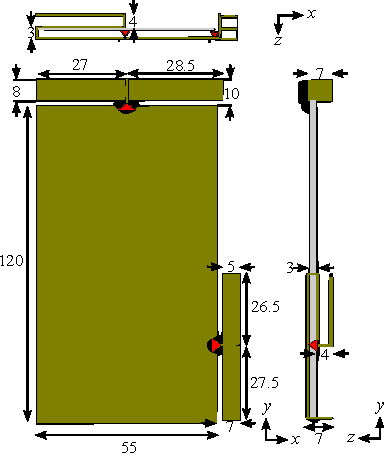
\includegraphics{img/tech_sol/monopole/tech_drawing}
        \caption{Technical drawing.}
        \label{fig:ant1technical}
    \end{subfigure}
    \hfill
    \begin{subfigure}[b]{0.49\linewidth}
        \centering
        \includegraphics{img/tech_sol/schematic_tuning_1}\\[1cm]
\footnotesize
        \begin{tabular}{|l|l|l|l|}
            \hline
            & $C_1$ & $L_1$ & $C_2$ \\
            \hline
            Top antenna & \SI{3.02}{pF} & \SI{7.99}{nH} & $[0.3,2.9]\,$pF\\
            Side antenna & \SI{1.81}{pF} & \SI{5.27}{nH} & $[0.3,2.9]\,$pF\\
            \hline
        \end{tabular}
        \caption{Tuning/matching circuit.}
        \label{fig:ant1_tuning}
    \end{subfigure}
    \caption{Technical drawing and tuning circuit for the antenna.  The matching circuit is applied for both the top and the side antenna.}
    \label{fig:ant2techschem}
\end{figure}

%Single antenna description
The antenna design for both antennas is shown in Figure \ref{fig:an1technical}. Both antennas is designed from a basic folded monopole structure with 2 arms one for the low band and one for the high band. The antennas are almost identical with a few changes as a result of the restrictions on the ground clearance.
The antennas are designed to take full advantage of the ground clearance requirements in all directions. This is done in order to obtain the highest possible bandwidth in the low band and high band. 


%MIMO
Going from the top antenna to the side antenna the ground clearance decreases from \SI{10}{mm} to \SI{7}{mm}. To compensate for the decrease in ground clearance the length of both the low band and high band arms are adjusted to meet the bandwidth requirements.

\begin{figure}[htbp]
   \begin{subfigure}[b]{0.32\linewidth}
        \centering
        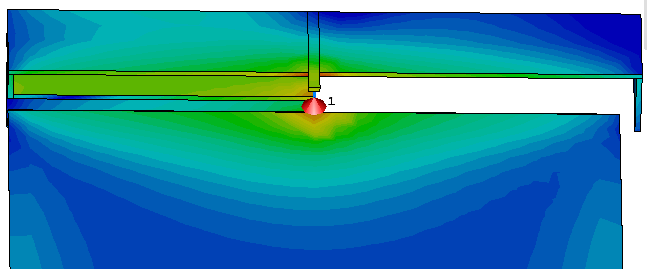
\includegraphics[width=\linewidth]{img/tech_sol/monopole/sc_800}
        \caption{Surface current for \SI{800}{MHz}}
        \label{fig:ant1_sc800}
    \end{subfigure}
    \hfill
    \begin{subfigure}[b]{0.32\linewidth}
        \centering
        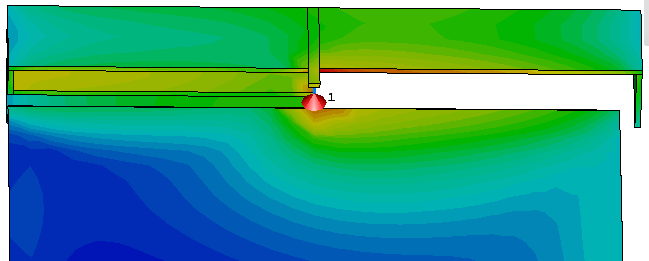
\includegraphics[width=\linewidth]{img/tech_sol/monopole/sc_1800}
        \caption{Surface current for \SI{1800}{MHz}}
        \label{fig:ant1_sc1800}
    \end{subfigure}
    \hfill
    \begin{subfigure}[b]{0.32\linewidth}
        \centering
        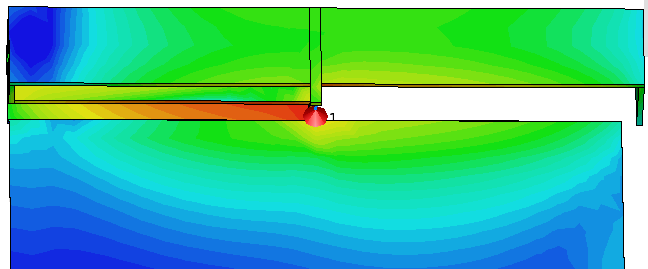
\includegraphics[width=\linewidth]{img/tech_sol/monopole/sc_2400}
        \caption{Surface current for \SI{2400}{MHz}}
        \label{fig:ant1_sc2400}
    \end{subfigure}
    \caption{Surface currents at each resonance with $C_2=\SI{0.3}{pF}$.}
    \label{fig:ant1_sc}
\end{figure}

\begin{figure}[htbp]
    \centering
    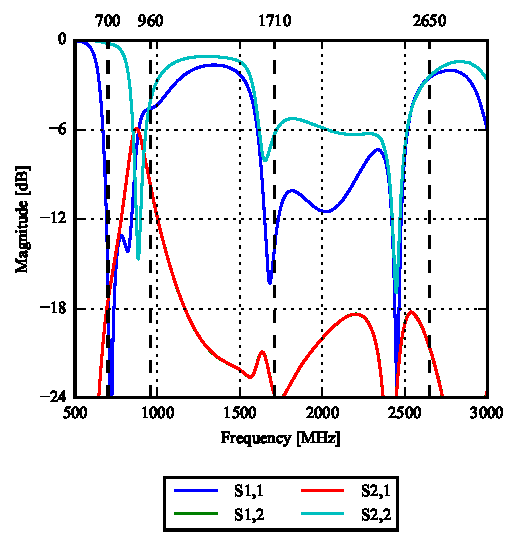
\includegraphics{img/tech_sol/monopole/ant1_sparam}
    \caption{S-parameters with $C_2=\SI{0.3}{pF}$ for both antennas.}
    \label{fig:ant1surfaces}
\end{figure}

The S11 and S22 sweeps \ref{fig:sparam_mono} shows that both antennas almost covers the desired bandwidth specified in the requirements \ref{cha:reqspec}. However at approx. \SI{2500}{MHz} to \SI{2650}{MHz} both antennas are \SI{-1}{dB} to \SI{-3}{dB} lower than required. The return loss from the side antenna  
\ref{fig:ant1_s22} also shows a lower level that desired, at approx \SI{-5}{dB}. From the requirement specification \ref{cha:reqspec} it is specified that for the low band the minimum channel bandwidth should be \SI{80}{MHz} and for the high band \SI{720}{MHz}. The channel bandwidth for both antennas are shown in Table. \ref{tab:asd}

\subsection{Bandwidth}

    \begin{table}
        \centering
        \begin{tabular}{|l|l|r|r|r|}
            \hline
            Antenna & Band & Start [MHz] & Stop [MHz] & Bandwidth [MHz] \\
            \hline
            Top     & Low  & 680         & 1011       & 331 \\
            Side    & Low  & 818         & 909        & 91 \\
            \hline
            Top     & High & 1590        & 2527       & 937 \\
            Side    & High & 1850        & 2533       & 683 \\
            \hline
        \end{tabular}
        \caption{Maximum bandwidth obtained in the low and high band for the top and the side antenna, respectively.}
        \label{tab:bw_sol2}
    \end{table}

\begin{figure}[htbp]
   \begin{subfigure}[b]{0.49\linewidth}
        \centering
        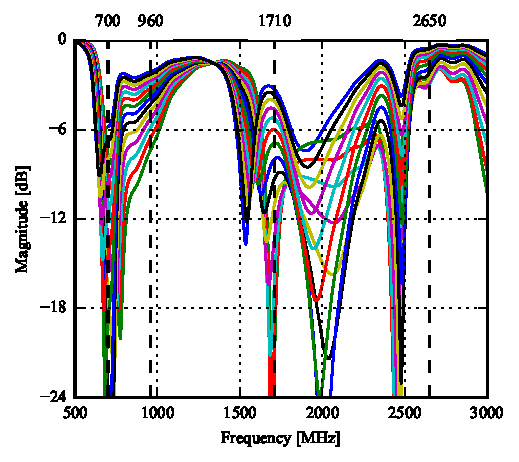
\includegraphics{img/tech_sol/monopole/s11}
        \caption{S11 plot for the bottom antenna.}
        \label{fig:ant1_s11}
    \end{subfigure}
    \hfill
    \begin{subfigure}[b]{0.49\linewidth}
        \centering
        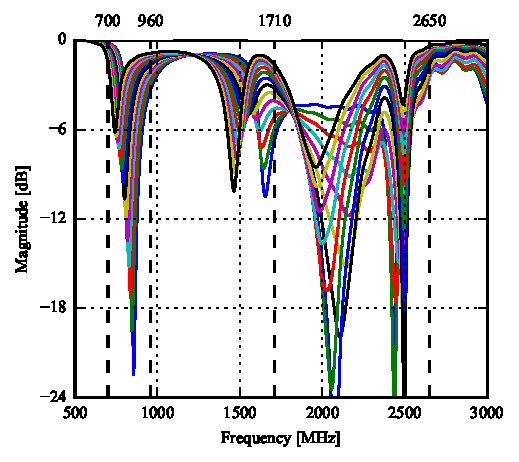
\includegraphics{img/tech_sol/monopole/s22}
        \caption{S22 plot for the side antenna.}
        \label{fig:ant1_s22}
    \end{subfigure}
~
    \begin{subfigure}[b]{0.49\linewidth}
        \centering
        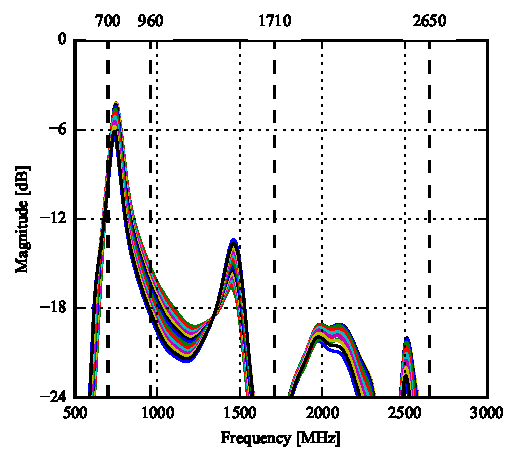
\includegraphics{img/tech_sol/monopole/s21-s11}
        \caption{$S_{21}$ with $C_2$ = \SI{0.3}{pF} and $C_1$ varying from \SI{0.3}{pF} to \SI{2.9}{pF}.}
        \label{fig:ant1_s11}
    \end{subfigure}
    \hfill
    \begin{subfigure}[b]{0.49\linewidth}
        \centering
        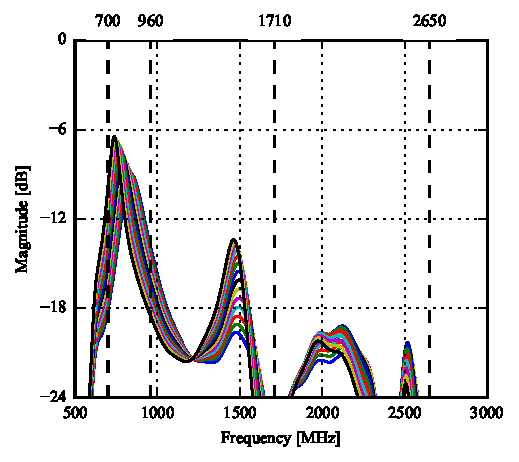
\includegraphics{img/tech_sol/monopole/s21-s22}
        \caption{$S_{21}$ with $C_2$ = \SI{0.3}{pF} and $C_1$ varying from \SI{0.3}{pF} to \SI{2.9}{pF}.}
        \label{fig:ant1_s22}
    \end{subfigure}
    \caption{Parameter sweep for tuning the shunt capacitor of each antenna, $C_1$ and $C_2$ for port 1 and 2, respectively. Port 1 is the top antenna and port 2 is the side antenna.}
    \label{fig:sparam_mono}
\end{figure}


